\documentclass[11pt,a4paper,oneside]{mwart}
%cała konfiguracja TeXa
\usepackage[utf8]{inputenc}

\def \MYHEADER {Planowanie działań i~ruchu robotów}
\def \MYTITLE {Wyszukiwanie ścieżki w~labiryncie\\za pomocą algorytmów \\przeszukiwania wszerz \\oraz\\przeszukiwania w~głąb}
\def \MYPDFTITLE {Plan.dzial.i.ruch.rob}

\def \MYPDFDATE {\today}

\def \MYAUTHOR {\emph{Autorzy:}\\Wojciech \textsc{Matkowski}\\Piotr \textsc{Mika}\\Paweł \textsc{Ruciński}}
\def \MYPDFAUTHOR {Piotr Mika}

\def \MYLECTURER {\emph{Prowadzący:} \\dr~in\.z. I.~\textsc{Dulęba}}

\def \MYLSTSETLANGUAGE {c++}

\def \MYLSTSETFRAME {lines}
						%none, %single, 

\def \MYLSTSETKEYWORDS {} 

%konfiguracja bez treści, aby podłączać do innych plików

\usepackage[OT4,plmath,MeX]{polski}


\usepackage{indentfirst} % polski zwyczaj dla wciec akapitowych
\usepackage{graphicx}
\graphicspath{{../}}
\usepackage[decimalsymbol=comma]{siunitx}
\usepackage{url}
\usepackage{pdflscape} 
\usepackage{subfigure}

\usepackage{wrapfig}
\usepackage[top=3cm, bottom=3cm, left=2cm, right=2cm]{geometry}

%\oddsidemargin 0.5cm
%\evensidemargin -0.5cm

\usepackage{listings}
\renewcommand{\labelitemi}{$\circ$}
\renewcommand{\today}{\oldstylenums{\number\day}~\ifcase\month\or
  stycznia\or lutego\or marca\or kwietnia\or maja\or czerwca\or
  lipca\or sierpnia\or września\or października\or
  listopada\or grudnia\fi \space\oldstylenums{\number\year} r.}

\usepackage{caption}
\usepackage{color}
\usepackage{rotating}
\usepackage{floatflt}
\usepackage{float}
\newfloat{scheme}{pb}{htbp} % second argument was {plt}
\floatname{scheme}{Schemat}
\newfloat{plot}{pb}{htbp} % second argument was {plt}
\floatname{plot}{Wykres}
\renewcommand*{\figurename}{Rysunek}
\renewcommand*{\tablename}{Tabela} 
\renewcommand*{\lstlistingname}{Kod}
\captionsetup{labelsep=period}
\usepackage{lscape}

\usepackage{amsmath}
\usepackage{mathtools}

\definecolor{dkgreen}{rgb}{0,0.5,0}
\definecolor{dkblue}{rgb}{0,0,0.7}
\definecolor{gray}{rgb}{0.5,0.5,0.5}
\definecolor{ltgray}{rgb}{0.8,0.8,0.8}
\definecolor{mauve}{rgb}{0.58,0,0.82}
\definecolor{maroon}{rgb}{0.5,0,0}

\newcommand{\HRule}{\rule{\linewidth}{0.5mm}}
\newcommand{\linia}{\rule{\linewidth}{0.1mm}}

\usepackage[ 
	pdftitle=\MYPDFTITLE,
	pdfauthor=\MYPDFAUTHOR,
	bookmarks=true, 
	bookmarksnumbered=false, 
	unicode=true, 
	pdftex, 
	pdfnewwindow=true,
	colorlinks=true,
	linkcolor=blue,
	hidelinks
]{hyperref} 


\usepackage[Procedura]{algorithm}
\usepackage{algorithmic}
\renewcommand\listalgorithmname{Spis procedur}
\makeatletter
\renewcommand\thealgorithm{\thechapter\@arabic\c@algorithm.}
\makeatother
\renewcommand\algorithmicforall{\textbf{Dla wszystkich}}
\renewcommand\algorithmicdo{\textbf{wykonaj:}}
\renewcommand\algorithmicendfor{\textbf{koniec.}}
\renewcommand\algorithmicif{\textbf{Jeżeli}}
\renewcommand\algorithmicthen{\textbf{to:}}
\renewcommand\algorithmicendif{\textbf{koniec.}}
\renewcommand\algorithmicelse{\textbf{w przeciwnym wypadku:}}
\renewcommand\algorithmicreturn{\textbf{powrót:}}
\renewcommand\algorithmicrequire{\textbf{Wymagane:}}
\renewcommand\algorithmicwhile{\textbf{Dopóki}}
\renewcommand\algorithmicendwhile{\textbf{koniec.}}
\setlength{\algorithmicindent}{2em}



\lstset{
	language=\MYLSTSETLANGUAGE,
	frame=\MYLSTSETFRAME,
	morekeywords=\MYLSTSETKEYWORDS,
	basicstyle=\footnotesize,
	numbers=left, 
	numberstyle=\tiny\color{gray},
	stepnumber=1,
	columns=fixed,
	numbersep=20pt, 
	backgroundcolor=\color{white}, 
	showspaces=false, 
	showstringspaces=true, 
	showtabs=false, 
	rulecolor=\color{ltgray},
	tabsize=4,
	breakatwhitespace=true,
	breakindent=30pt,
	breaklines=true,
	breakautoindent=true,
	prebreak=\mbox{{\color{red}$\hookleftarrow$}},
	postbreak=\mbox{{\color{red}$\hookrightarrow$}}\space,
	keywordstyle=\color{dkblue},
	commentstyle=\color{red},
	stringstyle=\color{dkgreen},
	identifierstyle=\color{maroon},
	morekeywords=_MY_MACRO_LSTSET_KEYWORDS
}


%\renewcommand{\thefootnote}{_MY_MACRO_FOOTNOTE}
%define _MY_MACRO_FOOTNOTE $\dagger$
						  %\fnsymbol{footnote}
						  % $\bullet${}
						  %\Roman{footnote}
						  %\alph{footnote}

\renewcommand{\thefootnote}{\roman{footnote}}
%\fnsymbol{footnote}}
\makeatletter 
\def\@fnsymbol#1{\ensuremath{\ifcase#1\or %*\or przeniesione z
\dagger\or \ddagger\or
   \mathsection\or \mathparagraph\or \|\or *\or %przeniesione tu
   **\or \dagger\dagger
   \or \ddagger\ddagger \else przypis\fi}}
%  \or \ddagger\ddagger \else\@ctrerr\fi}} %błąd jak jest za dużo i skończą się znaczki
\makeatother





\begin{document}

\begin{titlepage}
\begin{center}
\textsc{\Large \MYHEADER }\\[3cm]
\centering{\HRule \\[0.5cm]}
{\LARGE  \textsc{ \MYTITLE }\\[0.4cm]}
\centering{\HRule \\[1.5cm]}
\begin{minipage}[b]{0.4\textwidth}
\begin{flushleft} \large
\MYAUTHOR
\end{flushleft}
\end{minipage}
\begin{minipage}[b]{0.4\textwidth}
\begin{flushright} \large
\MYLECTURER
\end{flushright}
\end{minipage}
\vfill
{\large \MYPDFDATE}
\end{center}
\end{titlepage}



\newpage
\thispagestyle{empty}
~~~~~~~~~~~~~~
\newpage

\setcounter{tocdepth}{3}
\tableofcontents
\newpage

\section{Wstęp}

Robot mobilny, poza możliwością poruszania się musi także mieć umiejętność wybrania swojej trasy.
Ścieżka ta musi gwarantować bezkolizyjność. 
Zwykle też chcemy minimalizować koszty wyrażany np. jako ilość energii potrzebna do przebycia trasy 
lub czas jej pokonania.
W~celu uproszczenia obliczeń oraz zapisania przestrzeni (środowiska) w~postaci cyfrowej przedstawiamy 
otoczenie w~postaci grafu. 
Poszczególne krawędzie grafu oznaczają ścieżki, których przebycie nie niesie za sobą żadnych 
,,niespodzianek''\footnote{Przetworzenie przestrzeni na graf, oraz ustalenie wag krawędzi jest innym 
zadaniem, nie rozpatrywanym w~tej pracy.}.
Oznacza to, że planowanie ścieżki sprowadza się do znalezienia jej w~grafie.

Celem projektu jest stworzenie programu wizualizującego wyszukiwanie ścieżki w~labiryncie -- grafie.

\subsection{Omówienie algorytmów}

Metody przeszukiwania grafów można podzielić na dwie podstawowe grupy: 
przeszukiwania ślepe (ang. \emph{blind search}) oraz przeszukiwania zachłanne i~heurystyczne.

Przeszukiwania ślepe są najprostszymi algorytmami. 
Nie uwzględniają one żadnych zależności dotyczących wag krawędzi.
Takimi algorytmami są \emph{przeszukiwanie w~głąb} oraz \emph{przeszukiwanie wszerz}.

Algorytmy zachłanne i~heurystyczne zwykle znajdują optymalną ścieżkę w~grafie 
(np. alg. Dijkstry), a~używanie heurystyki (np. alg. A*) powoduje zdecydowane przyspieszenie obliczeń.

\subsubsection{Przeszukiwanie wszerz}
W celu znalezienia ścieżki od wierzchołka~A do wierzchołka~B algorytm wykonuje następujące kroki:
\begin{algorithm}
\caption{Przeszukiwanie wszerz}
\label{algorytm_wszerz}
\begin{algorithmic}[1]
\STATE{Dodaj wierzchołek A~do kolejki.}
\WHILE{kolejka nie jest pusta}
	\STATE{Pobierz \underline{pierwszy} wierzchołek z~kolejki.}
	\FORALL{wierzchołków połączonych z~bieżącym}
		\IF{wierzchołek nie był odwiedzony}
			\STATE{Dodaj wierzchołek na \underline{koniec} kolejki.}
		\ENDIF
	\ENDFOR
\ENDWHILE
\end{algorithmic}
\end{algorithm}

Taka metodyka powoduje dotarcie do każdego z~wierzchołków w~grafie, jeśli tylko istnieje ścieżka do niego.
Dodatkowo, jeśli wagi krawędzi są równe to algorytm ten jest równoważny z~algorytmem Dijkstry i~znajduje 
najkrótszą ścieżkę.
Jeśli interesuje nas dowolna ścieżka od~A do~B algorytm może zakończyć pracę w momencie dotarcia do punktu~B.


\subsubsection{Przeszukiwanie w~głąb}
Algorytm ten jest bardzo zbliżony do przeszukiwania wszerz, jedynie różni się tylko kolejnością pobierania 
wierzchołków z~kolejki.
\begin{algorithm}
\caption{Przeszukiwanie w~głąb}
\label{algorytm_w_glab}
\begin{algorithmic}[1]
\STATE{Dodaj wierzchołek A~do kolejki.}
\WHILE{kolejka nie jest pusta}
	\STATE{Pobierz \underline{ostatni} wierzchołek z~kolejki.}
	\FORALL{wierzchołków połączonych z~bieżącym}
		\IF{wierzchołek nie był odwiedzony}
			\STATE{Dodaj wierzchołek na \underline{koniec} kolejki.}
		\ENDIF
	\ENDFOR
\ENDWHILE
\end{algorithmic}
\end{algorithm}

Powoduje to jednak możliwość wystąpienia sytuacji w~której znaleziona ścieżka będzie dłuższa niż optymalna.

\begin{figure}[!h]
\centering
\framebox{
\includegraphics[angle=0,width=0.3\textwidth]{img/petla.png}}
\caption{Ścieżka nieoptymalna znaleziona przeszukiwaniem w~głąb (start -- zielony, stop -- czerwony)\label{petla}}
\end{figure}

\subsection{Typy labiryntów}
Robot porusza się w~przestrzeni dwuwymiarowej z~przeszkodami. 
W~tym projekcie przyjęto metodę nałożenia siatki na przestrzeń. 
Powoduje to powstanie dwóch typów punktów: dozwolonych i~zabronionych. 
Z~punktu dozwolonego można przejść na sąsiadujące z~nim punkty dozwolone.

Labiryntem nazywamy obszar w~którym znalezienie ścieżki (przez człowieka) jest utrudnione.
Zwykle wynika to z~dużej ilości rozwidleń danej ścieżki. 
Rozwidlenia te dodatkowo nie prowadzą do punktu końcowego. 
Typ mapy (labirynt lub nie) nie ma żadnego wpływu na działanie algorytmu, gdyż algorytm w~przeciwieństwie do 
człowieka potrafi zapamiętać dowolnie długa i~skomplikowaną ścieżkę.

\subsubsection{Wpływ grubości ścieżki}
\begin{figure}[!htp]
\begin{center}$
\begin{array}{cp{2cm}c}
\framebox{
\includegraphics[angle=0,width=0.3\textwidth]{img/podwojna_g.png}} & &
\framebox{
\includegraphics[angle=0,width=0.3\textwidth]{img/podwojna_s.png}}
\end{array}$
\end{center}
\caption{,,Zapętlenie'' przeszukiwania w~głąb (po lewej) w~porównaniu 
do przeszukiwania wszerz(po prawej)\label{podwojna}}
\end{figure}
Badane algorytmy nie uwzględniają grubości ścieżki przechodząc taką ścieżkę kilka razy.
Powoduje to wydłużanie czasu obliczeń, a~w~przypadku przeszukiwania w~głąb znaleziona ścieżka może być
zawinięta.


\section{Realizacja}
Program został napisany w języku \emph{C++} przy użyciu biblioteki \emph{Qt}.
Obrazy są obsługiwane za pomocą klasy \emph{QImage}, a~graficzny interfejs jest zbudowany przy pomocy 
technologii \emph{Qt Widgets}.
\emph{Qt} dostarcza programiście dodatkowe elementy, które rozszerzają język \emph{C++} o nowe mechanizmy.
Są to makra \lstinline!Q_OBJECT! oraz mechanizm sygnałów i~slotów.
Te dodatkowe elementy wymuszają niestandardową kompilację, która jest omówiona 
w~dodatku \ref{sec_uruchomienie}. na stronie \pageref{sec_uruchomienie}.

\lstinline!Q_OBJECT! pozwala rozszerzyć możliwości każdej klasy o dodatkowe, zestandaryzowane mechanizmy
biblioteki \emph{Qt}. Są one potrzebne do lepszego zarządzania pamięcią oraz dla mechanizmu sygnałów i~slotów.

Dzięki sygnałom i~slotom można łączyć dowolne zdarzenia w~programie. 
W~ten sposób obsługiwany jest interfejs użytkownika.
Zdarzenia wywoływane akcjami użytkownika uruchamiają odpowiednie funkcje w klasie opisującej 
główne okno programu. 
Na schemacie \ref{przeplyw}. przedstawiono komunikację wewnątrz programu.

\begin{scheme}[!h]
\centering
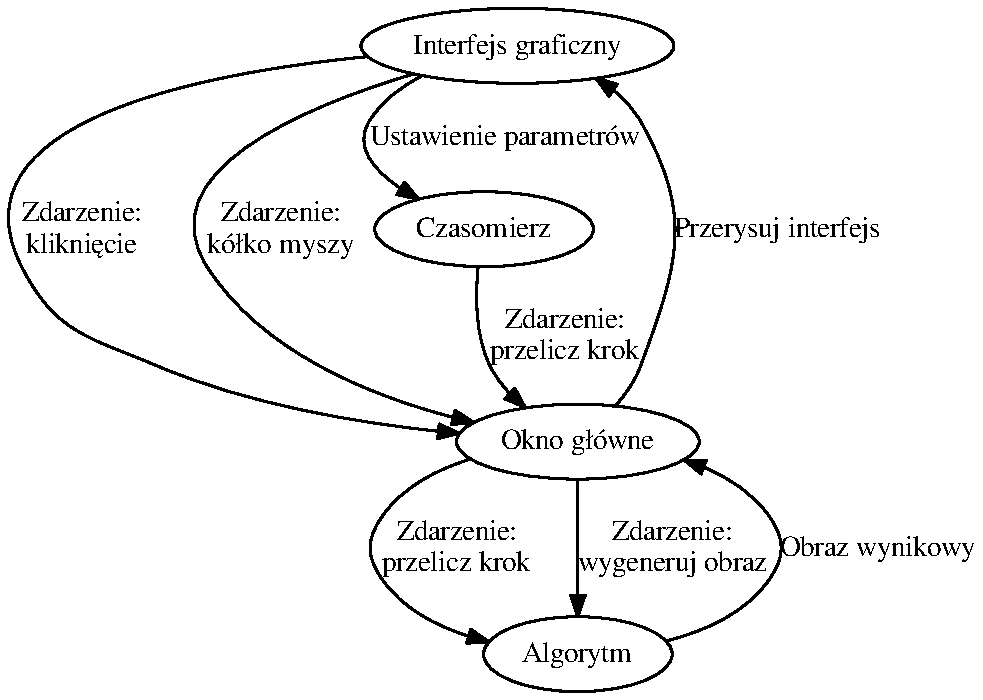
\includegraphics[angle=0,width=0.7\textwidth]{img/przeplyw.pdf}
\caption{Przepływ danych i zdarzeń w programie\label{przeplyw}}
\end{scheme}

\section{Badania}
Badania przeprowadzono na zestawie zawierającym trzy labirynty, przygotowane przy pomocy internetowego generatora \url{http://hereandabove.com/maze/mazeorig.form.html}:
\begin{enumerate}
\item Łatwy (\url{src/labirynty/maly_latwy.png}), \label{en_lat}
\item Trudny (\url{src/labirynty/maly_trudny.png}), \label{en_tr}
\item Łatwy powiększony (\url{src/labirynty/maly_latwy_powiekszony.png}). \label{en_lat_pow}
\end{enumerate}
Zostały one przygotowane tak, aby posiadały pewne cechy wspólne:
labirynt~\ref{en_lat}.~i~\ref{en_tr}. mają taką samą ilość punktów do odwiedzenia.
Labirynt łatwy powiększony~(\ref{en_lat_pow}.) jest labiryntem~\ref{en_lat}. przeskalowanym dwukrotnie.
Oznacza to, że każda ścieżka jest podwójnej grubości.

Badano jak zachowuje się ilość elementów w kolejce oraz jaką długość ma ścieżka do punktu odwiedzanego
w~danym kroku.

\subsection{Labirynt łatwy}
Labirynt został określona jako łatwy, gdyż zawiera dużo prostych ścieżek i~mało rozgałęzień.
Poniższe obrazy przedstawiają kroki pracy algorytmu, kolor oznacza kolejność odwiedzenia punktów:
niebieski -- początek, zielony -- środek, czerwony -- koniec (punkty odwiedzone jako ostatnie).

\begin{figure}[!htp]
\begin{center}$
\begin{array}{llll}
\includegraphics[angle=0,width=0.225\textwidth]{img/latwy_w_glab/easy_maze_0.png} & 
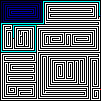
\includegraphics[angle=0,width=0.225\textwidth]{img/latwy_w_glab/easy_maze_1.png} & 
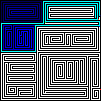
\includegraphics[angle=0,width=0.225\textwidth]{img/latwy_w_glab/easy_maze_2.png} & 
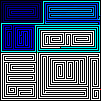
\includegraphics[angle=0,width=0.225\textwidth]{img/latwy_w_glab/easy_maze_3.png}
\\
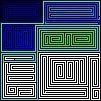
\includegraphics[angle=0,width=0.225\textwidth]{img/latwy_w_glab/easy_maze_4.png} & 
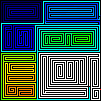
\includegraphics[angle=0,width=0.225\textwidth]{img/latwy_w_glab/easy_maze_5.png} & 
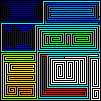
\includegraphics[angle=0,width=0.225\textwidth]{img/latwy_w_glab/easy_maze_6.png} & 
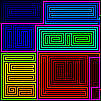
\includegraphics[angle=0,width=0.225\textwidth]{img/latwy_w_glab/easy_maze_7.png}
\end{array}$
\end{center}
\caption{Przeszukiwanie w głąb -- labirynt łatwy}
\end{figure}

\begin{figure}[!htp]
\begin{center}$
\begin{array}{llll}
\includegraphics[angle=0,width=0.225\textwidth]{img/latwy_wszerz/easy_maze_0.png} & 
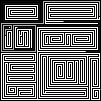
\includegraphics[angle=0,width=0.225\textwidth]{img/latwy_wszerz/easy_maze_1.png} & 
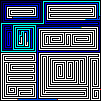
\includegraphics[angle=0,width=0.225\textwidth]{img/latwy_wszerz/easy_maze_2.png} & 
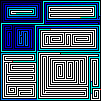
\includegraphics[angle=0,width=0.225\textwidth]{img/latwy_wszerz/easy_maze_3.png}
\\
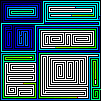
\includegraphics[angle=0,width=0.225\textwidth]{img/latwy_wszerz/easy_maze_4.png} & 
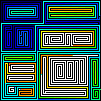
\includegraphics[angle=0,width=0.225\textwidth]{img/latwy_wszerz/easy_maze_5.png} & 
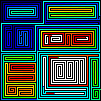
\includegraphics[angle=0,width=0.225\textwidth]{img/latwy_wszerz/easy_maze_6.png} & 
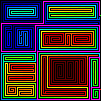
\includegraphics[angle=0,width=0.225\textwidth]{img/latwy_wszerz/easy_maze_7.png}
\end{array}$
\end{center}
\caption{Przeszukiwanie wszerz -- labirynt łatwy}
\end{figure}

Powyższe obrazy przedstawiają kilka kroków przeszukiwania obydwoma badanymi algorytmami.

\subsection{Labirynt trudny}

Trudność labiryntu wynika z dużej ilości załamań i rozgałęzień ścieżek.

\begin{figure}[!htp]
\begin{center}$
\begin{array}{llll}
\includegraphics[angle=0,width=0.225\textwidth]{img/trudny_w_glab/hard_maze_0.png} & 
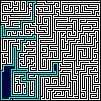
\includegraphics[angle=0,width=0.225\textwidth]{img/trudny_w_glab/hard_maze_1.png} & 
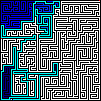
\includegraphics[angle=0,width=0.225\textwidth]{img/trudny_w_glab/hard_maze_2.png} & 
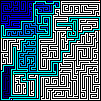
\includegraphics[angle=0,width=0.225\textwidth]{img/trudny_w_glab/hard_maze_3.png}
\\
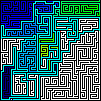
\includegraphics[angle=0,width=0.225\textwidth]{img/trudny_w_glab/hard_maze_4.png} & 
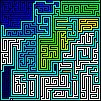
\includegraphics[angle=0,width=0.225\textwidth]{img/trudny_w_glab/hard_maze_5.png} & 
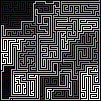
\includegraphics[angle=0,width=0.225\textwidth]{img/trudny_w_glab/hard_maze_6.png} & 
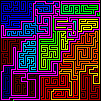
\includegraphics[angle=0,width=0.225\textwidth]{img/trudny_w_glab/hard_maze_7.png}
\end{array}$
\end{center}
\caption{Przeszukiwanie w głąb -- labirynt trudny}
\end{figure}

\begin{figure}[!htp]
\begin{center}$
\begin{array}{llll}
\includegraphics[angle=0,width=0.225\textwidth]{img/trudny_wszerz/hard_maze_0.png} & 
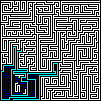
\includegraphics[angle=0,width=0.225\textwidth]{img/trudny_wszerz/hard_maze_1.png} & 
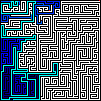
\includegraphics[angle=0,width=0.225\textwidth]{img/trudny_wszerz/hard_maze_2.png} & 
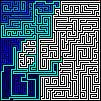
\includegraphics[angle=0,width=0.225\textwidth]{img/trudny_wszerz/hard_maze_3.png}
\\
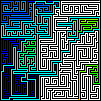
\includegraphics[angle=0,width=0.225\textwidth]{img/trudny_wszerz/hard_maze_4.png} & 
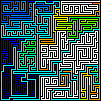
\includegraphics[angle=0,width=0.225\textwidth]{img/trudny_wszerz/hard_maze_5.png} & 
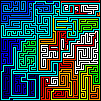
\includegraphics[angle=0,width=0.225\textwidth]{img/trudny_wszerz/hard_maze_6.png} & 
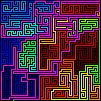
\includegraphics[angle=0,width=0.225\textwidth]{img/trudny_wszerz/hard_maze_7.png}
\end{array}$
\end{center}
\caption{Przeszukiwanie wszerz -- labirynt trudny}
\end{figure}

\subsection{Labirynt łatwy powiększony}
Jest to labirynt łatwy powiększony dwukrotnie.
Na obrazach można zaobserwować ,,szachownicę'' wewnątrz niektórych korytarzy. 
Oznacza to, że dany korytarz jest odwiedzany kolejny raz po odwiedzeniu innego obszaru.
Zazwyczaj jest to powrót ze ślepej ścieżki. 


\begin{figure}[!htp]
\begin{center}$
\begin{array}{llll}
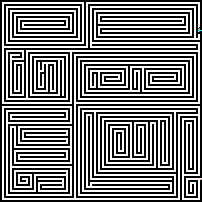
\includegraphics[angle=0,width=0.225\textwidth]{img/latwy_powiekszony_w_glab/maze_0.png} & 
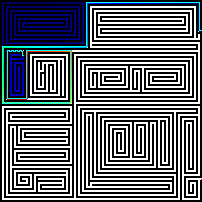
\includegraphics[angle=0,width=0.225\textwidth]{img/latwy_powiekszony_w_glab/maze_1.png} & 
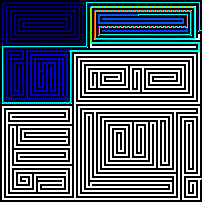
\includegraphics[angle=0,width=0.225\textwidth]{img/latwy_powiekszony_w_glab/maze_2.png} & 
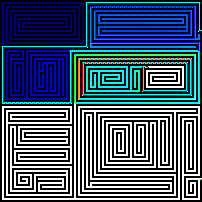
\includegraphics[angle=0,width=0.225\textwidth]{img/latwy_powiekszony_w_glab/maze_3.png}
\\
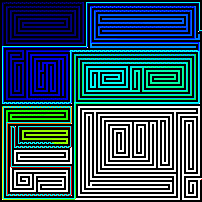
\includegraphics[angle=0,width=0.225\textwidth]{img/latwy_powiekszony_w_glab/maze_4.png} & 
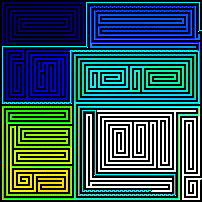
\includegraphics[angle=0,width=0.225\textwidth]{img/latwy_powiekszony_w_glab/maze_5.png} & 
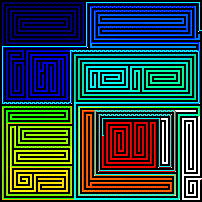
\includegraphics[angle=0,width=0.225\textwidth]{img/latwy_powiekszony_w_glab/maze_6.png} & 
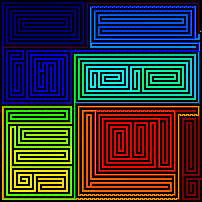
\includegraphics[angle=0,width=0.225\textwidth]{img/latwy_powiekszony_w_glab/maze_7.png}
\end{array}$
\end{center}
\caption{Przeszukiwanie w głąb -- labirynt łatwy powiększony}
\end{figure}

\begin{figure}[!htp]
\begin{center}$
\begin{array}{llll}
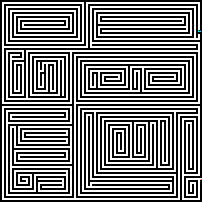
\includegraphics[angle=0,width=0.225\textwidth]{img/latwy_powiekszony_wszerz/maze_0.png} & 
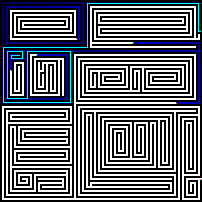
\includegraphics[angle=0,width=0.225\textwidth]{img/latwy_powiekszony_wszerz/maze_1.png} & 
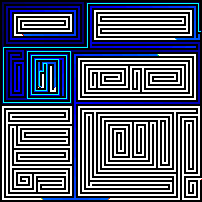
\includegraphics[angle=0,width=0.225\textwidth]{img/latwy_powiekszony_wszerz/maze_2.png} & 
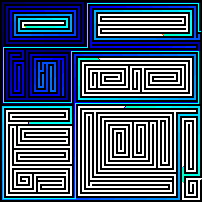
\includegraphics[angle=0,width=0.225\textwidth]{img/latwy_powiekszony_wszerz/maze_3.png}
\\
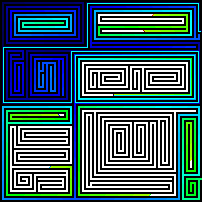
\includegraphics[angle=0,width=0.225\textwidth]{img/latwy_powiekszony_wszerz/maze_4.png} & 
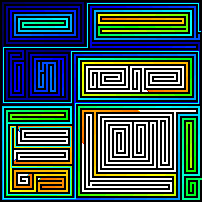
\includegraphics[angle=0,width=0.225\textwidth]{img/latwy_powiekszony_wszerz/maze_5.png} & 
\includegraphics[angle=0,width=0.225\textwidth]{img/latwy_powiekszony_wszerz/maze_6.png} & 
\includegraphics[angle=0,width=0.225\textwidth]{img/latwy_powiekszony_wszerz/maze_7.png}
\end{array}$
\end{center}
\caption{Przeszukiwanie wszerz -- labirynt łatwy powiększony}
\end{figure}



\subsection{Porównanie}
Podczas pracy algorytm korzysta z kolejki punktów do odwiedzenia oraz generuje ścieżkę do bieżącego punktu.
Wielkość tych obiektów podczas pracy przedstawiają poniższe wykresy.
\begin{figure}[!htp]
\begin{center}$
\begin{array}{ll}
\includegraphics[angle=0,width=0.49\textwidth]{img/latwy_kolejka.pdf} & 
\includegraphics[angle=0,width=0.49\textwidth]{img/latwy_sciezka.pdf}
\end{array}$
\end{center}
\caption{Długość kolejki i długość ścieżki -- labirynt łatwy}
\end{figure}

\begin{figure}[!htp]
\begin{center}$
\begin{array}{ll}
\includegraphics[angle=0,width=0.49\textwidth]{img/trudny_kolejka.pdf} & 
\includegraphics[angle=0,width=0.49\textwidth]{img/trudny_sciezka.pdf}
\end{array}$
\end{center}
\caption{Długość kolejki i długość ścieżki -- labirynt trudny}
\end{figure}

\begin{figure}[!htp]
\begin{center}$
\begin{array}{lll}
\includegraphics[angle=0,width=0.31\textwidth]{img/latwy_powiekszony_kolejka.pdf} & 
\includegraphics[angle=0,width=0.31\textwidth]{img/latwy_powiekszony_kolejka_log.pdf} & 
\includegraphics[angle=0,width=0.31\textwidth]{img/latwy_powiekszony_sciezka.pdf}
\end{array}$
\end{center}
\caption{Długość kolejki (skala liniowa i logarytmiczna) oraz długość ścieżki -- labirynt łatwy powiększony}
\end{figure}

W przypadku labiryntów o pojedynczej grubości ścieżki żaden z algorytmów nie wykazuje znaczącej przewagi.
Dodatkowo można zaobserwować ważną cechę przeszukiwania wszerz: gdy wagi wszystkich krawędzi są równe to jest
ono równoznaczne z algorytmem Dijkstry. 
Pokazuje to niemalejąca długość ścieżki do kolejno odwiedzanych punktów.

Jeśli zaś grubość ścieżki jest większa od~1, to pojawiają się cykle i~możliwość zawijania się ścieżki.
W takiej sytuacji algorytm przeszukiwania w~głąb tworzy bardzo długą kolejkę wynikającą 
z~dodania punktów wzdłuż takiego przejścia.
Możliwość tworzenia kolejki w~taki sposób powoduje, że ma ona dużo większą długość.

W przypadku przeszukiwania wszerz kolejka jest dłuższa o ok. współczynnik skalowania.

\section{Wnioski}

\begin{itemize}
\item Podstawowym parametrem różnicującym labirynty jest ich grubość ścieżki.\\~
\item Dla labiryntów o ścieżkach grubości jeden ciężko wskazać lepszy z algorytmów. 
Jedynie w przypadku wystąpienia cyklu przeszukiwanie w głąb może znaleźć nieoptymalną ścieżkę.\\~
\item Jeśli interesuje nas znalezienie dowolnej ścieżki do zadanego punktu żaden 
z~algorytmów nie gwarantuje jej szybszego znalezienia.\\~
\item Dla labiryntu z~grubymi ścieżkami przeszukiwanie w~głąb generuje dużo dłuższe kolejki.\\~
\item Czas procesora wykorzystywany na wizualizację jest porównywalny z czasem obliczeń algorytmów.\\~
\item Dla ogólnych zastosowań algorytm przeszukiwania wszerz jest lepszy.\\~
\end{itemize}

\appendix

\section{Uruchomienie aplikacji\label{sec_uruchomienie}}
\begin{figure}[!h]
\centering
\includegraphics[angle=0,width=1\textwidth]{img/gui.png}
\caption{Interfejs programu\label{gui}}
\end{figure}

Po uruchomieniu aplikacji należy wczytać obraz, wybrać typ algorytmu i~określić, 
czy program ma generować plik statystyk.
Pozostałe opcje można ustawiać podczas pracy.

\subsection{Kompilacja ze źródeł}
Kompilację programu najłatwiej przeprowadzić w~środowisku \emph{Qt Creator}. 
Jest ono dostępne dla platform Windows, Linux, Mac i innych.
Po zaimportowaniu projektu używamy przycisku ,,build'' i otrzymujemy gotową aplikację.
Środowisko samo wykona wszystkie etapy kompilacji.
Kompilacja projektu w~\emph{Qt} składa się z kilku etapów: 
\begin{itemize}
\item \textsc{qmake}: na podstawie pliku \emph{*.pro} jest tworzony i uruchamiany plik Makefile, 
w~którym zawarte są kolejne operacje,
\item \textsc{uic}: przetwarza pliki \emph{*.ui} (opisujące interfejs graficzny) na pliki \emph{*.hpp},
\item \textsc{moc}: przetwarza pliki \emph{*.hpp}, rozwijając makra \lstinline!Q_OBJECT! 
oraz generując kod sygnałów i slotów,
\item \textsc{g++}: wygenerowane pliki są kompilowane kompilatorem języka \emph{C++}.
\end{itemize}


\end{document}

